\chapter{Einleitung}
blablablabla(\cite{Adler}, Seite 2)\\\\\\
Test\cite{Adler.2013}
\section{Quelltext}

Nachfolgend der \autoref{lst:helloworld}.\\
test\cite{Adler}

Die nachfolgende \autoref{img:beispielbild} demonstriert

\begin{figure}[H]
	\centering
	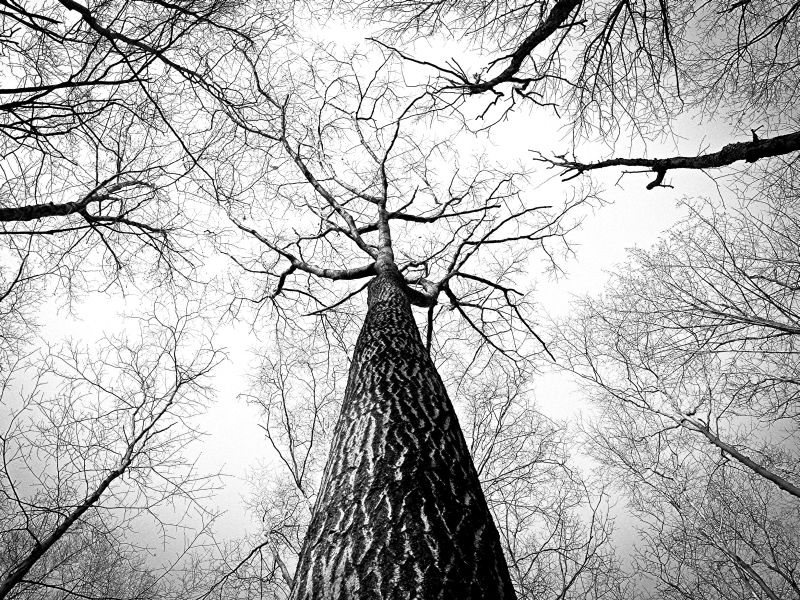
\includegraphics[width=0.7\textwidth]{resources/example}
	\caption{Beispielbild {\cite{PEXELS2015}}}
	\label{img:beispielbild}
\end{figure}

\begin{lstlisting}[caption={Hello World}, captionpos=b, label={lst:helloworld}]
/**
* The HelloWorldApp class implements an application that
* simply prints "Hello World!" to standard output.
*/
class HelloWorldApp {
	public static void main(String[] args) {
		System.out.println("Hello World!"); // Display the string.
	}
}
\end{lstlisting}
\blindtext
